\documentclass[12pt]{article}
\usepackage[colorinlistoftodos]{todonotes}
\usepackage{amsmath}
\usepackage{amssymb}
\usepackage{bm}
\usepackage{enumerate}
\usepackage{fancyvrb}
\usepackage[top=1in, bottom=1in, left=1in, right=1in]{geometry}
\usepackage{hyperref}
\usepackage{placeins}
\usepackage{tikz}
\usepackage{tikzsymbols}
\usepackage{todonotes}
\usepackage{bbm}
\usepackage{color}
\usepackage{mathrsfs}
\usepackage{enumitem}

% \renewcommand{\theenumi}{\roman{enumi}}
\newcommand{\rmn}[1]{{\textcolor{blue}{\bf [{\sc rmn:} #1]}}}
\DeclareMathOperator*{\argmax}{arg\,max}

\usetikzlibrary{positioning,calc}
%%%%%%%%%
\usepackage[most]{tcolorbox}
\newtcolorbox[]{solution}[1][]{%
    breakable,
    enhanced,
    colback=white,
    title=Solution,
    #1
}
%%%%%%%%%%
\title{10-403 Deep Reinforcement Learning and Control\\
  Assignment 3: Model-Free Learning\\
  Spring 2019\\
}

\date{February 15th, 2019\\
  \hspace{1cm}\\
Due March 1st, 2019}

\begin{document}

\maketitle
\noindent
\section*{Instructions}

You may work in teams of \textbf{2} on this assignment. \textbf{Only one person should submit the writeup and code on Gradescope.} Additionally you should upload your code to Autolab, please make sure the same person who submitted the writeup and code to Gradescope is the one who submits it to Autolab.  Make sure you \textbf{mark your partner as a collaborator on Gradescope and form teams on Autolab} and that both names are listed in the writeup.  Writeups should be typeset in Latex (using the template we provide) and submitted as PDF. All code, including auxiliary scripts used for testing should be
submitted with a README.

\section*{Introduction}

% what is the goal of this section.
In Homework 2, you learned about and implemented various model-based techniques to solve MDPs. These ``planning'' techniques work well when we have access to a model of the environment; however getting access to such a model is often unfeasible. In this Homework, you will explore an alternative to the model-based regime, i.e. model-free learning. 
In particular, you will learn about Temporal Difference learning and its variants, and implement a version of TD learning called Q-learning. We will look at implementing Q learning with both tabular methods and deep function approximators. 

You will work with the OpenAI Gym environments, and learn how to train a Q-network from state inputs on a gym environment. The goal is to understand and implement some of the techniques that were found to be important in practice to stabilize training and achieve better performance. We also expect you to get comfortable using Tensorflow or Keras to experiment with different architectures, and understand how to analyze your network's final performance and learning behavior. 


\section*{Question 1 \textbf{[10 pts]}}
The objective of this question is to understand different Bellman equations, their strengths and limitations.
\subsection*{Question 1.a \textbf{[6 pts]}} Consider the Bellman Equation for Value function,
$$
    V(s_1) = \max_{a_1} \left( R(s_1,a_1) + \gamma \sum_{s_2}T(s_1, a_1, s_2)V(s_2) \right)
$$
If we continue expanding the value function $V(s_2)$ using its own bellman equation, we obtain a repeating structure as follows,
$$
     V(s_1) = \max_{a_1} \left( R(s_1,a_1) + \gamma \sum_{s_2}T(s_1, a, s_2) \max_{a_2} \left( R(s_2,a_2) + \gamma \sum_{s_3}T(s_2, a_2, s_3)V(s_3) \right) \right)
$$

There are a few more ways in which we can group this repeating sequence. First, we can capture the sequence starting at $R(s,a)$ and ending at $\max$, and observe that it too has a repeating substructure property, as shown,
$$
     V(s_1) = \max_{a_1} \underbrace {\left( R(s_1,a_1) + \gamma \sum_{s_2}T(s_1, a, s_2) \max_{a_2} \underbrace{\left( R(s_2,a_2) + \gamma \sum_{s_3}T(s_2, a_2, s_3)V(s_3) \right)}_{Q(s_2,a_2)} \right)}_{Q(s_1,a_1)}
$$
We'll call this repeating expression, the state-value function $Q(s,a)$ and use it to rewrite the bellman equation as,

$$
    Q(s_1,a_1) = R(s_1,a_1) + \gamma \sum_{s_2}T(s_1, a_1, s_2)\max_{a_2} Q(s_2, a_2)
$$

Next, we can capture another pattern by grouping the expression beginning at $\gamma$ and ending at $R(s,a)$, as shown,

$$
     V(s_1) = \max_{a_1} \left( R(s_1,a_1) + \underbrace{\gamma \sum_{s_2}T(s_1, a, s_2) \max_{a_2} \bigg( R(s_2,a_2) + \underbrace{\gamma \sum_{s_3}T(s_2, a_2, s_3)V(s_3)}_{C(s_2,a_2)}}_{C(s_1,a_1)} \bigg) \right)
$$

We'll call this repeating expression the continuation function $C(s,a)$, which can be written in terms of the value function as follows,

$$
    C(s_1,a_1) = \gamma\sum_{s_2}T(s_1,a_1,s_2)V(s_2)
$$

Your task is to \textcolor{red}{1.} derive the recurrence relation (bellman equation) for the Continuation function $C(s,a)$. \textcolor{red}{2.} Also, express the three functions in terms of each other, and $R(s,a)$, and fill up the following table. We've partially filled the table for you. 

\begin{center}
\begin{tabular}{ | c | c | c | c | }
 \hline
  & V(s) & Q(s,a) & C(s,a) \\ 
 \hline
 V(s) & V(s) = V(s)  & V(s) = $\max_{a} Q(s,a)$ & (i) \\  
 \hline
 Q(s,a) & (ii) & Q(s,a) = Q(s,a) & (iii)  \\
 \hline
 C(s,a) & $C(s,a) = \gamma\sum_{s'}T(s,a,s')V(s')$ & (iv) & C(s,a) = C(s,a)  \\
 \hline
\end{tabular}
\end{center}

\begin{solution}
i) $V(s) = \max_{a_{i}} R(s,a_{i}) + C(s,a_{i})$\\
ii)$Q(s,a) = R(s,a) + \gamma \sum_{s'} T(s,a,s')V(s')$ \\
iii)$Q(s,a) = R(s,a)  + C(s,a)$\\
iv)$C(s,a) = \gamma \sum_{s'} T(s,a,s')\max_{a'}Q(s',a')$
\end{solution}

\subsection*{Question 1.b \textbf{[4 pts]}}
Use the relation between the functions and your understanding of MDPs to answer if the following is true or false. Provide a brief explanation in one or two sentences. (No points will be awarded without any explanation)
\begin{enumerate}
    \item For computing the optimal action, knowing $Q(s,a)$ is better than knowing $V(s)$ if we lack knowledge of the transition function $T(s,a,s')$ or reward function $R(s,a)$.
    \item For computing the optimal action, knowing $V(s)$ is better than knowing $C(s,a)$ if we lack knowledge of the transition function $T(s,a,s')$ even if we know the reward function $R(s,a)$. 
\end{enumerate}

\begin{solution}
1. True.  If only V(s) is known, it is required that we know the dynamics in order to realize the optimal policy since we cannot know what action to take to move to a higher-valued state if we know only V(s) because we would not know what state we would end up in given any action.\\
2. False.  Knowing C(s,a) and R(s,a) gives Q(s,a) by (iii) in the previous problem, which is better than knowing V(s,a) by (1)
\end{solution}
% 2 + 2 + 4 + 4 = 12

\section*{Question 2 \textbf{[2+3+5+5=15 pts]}}
The objective of this question is to understand Importance Sampling and how it works. If you are able to correctly reason about the results you obtain in this question, you'll find yourself capable of drawing analogies on how importance sampling is applied to Monte Carlo Learning. \\

In this question, you'll find the expectation of the function $f(x) = \frac{3}{2}x^2(1 + x) \text{ } \forall\text{ } x \in \mathcal{R}$  with respect to the probability distribution function $p(x) = \frac{1}{2}(1 + x)$, $-1 \le x \le 1$ using different sampling methods. 

\begin{enumerate}
    \item Find the expectation and the variance of $f(x)$, analytically using the formulation \\ $\mathbb{E}_p[g(x)] = \int g(x)p(x)dx $ and $Var[g(x)] = \int (g(x) - \mathbb{E}_p[g(x)])^2p(x)dx $.
    \item Write a program to sample from the distribution $p(x)$ \footnote{Consider using the \href{https://docs.scipy.org/doc/scipy/reference/generated/scipy.stats.rv_continuous.html}{\underline{rv\_continuous}} class from scipy.stats to sample from a custom distribution} and compute the expectation and the variance of $f(x)$, using 10, 1000, 10000 samples. Report the values you obtain for each case. What do you observe as the number of samples increases (in terms of expectation and variance)?
    \item Now suppose you don't know how to sample from the distribution $p(x)$ but you know the ratio $r(x) = p(x)/q(x)$. Here, $q(x)$ is some proposal distribution, from which you know how to sample. Use importance sampling to compute the expectation and the variance of $f(x)$ using the following proposal distributions\footnote{Consider using \href{https://docs.scipy.org/doc/numpy-1.15.0/reference/generated/numpy.random.normal.html}{\underline{normal}} class from numpy.random to sample from a normal distribution} for 10, 1000, 10000 samples:
    \begin{itemize}
        \item $q(x) = N(3,1)$
        \item $q(x) = N(0,1)$
        \item $q(x) = \frac{15}{16}x^2(1+x)^2$
    \end{itemize}
    Report the values you obtain for each case. Which proposal distribution gives the lowest variance? Why do you think that is? Which of them converges the slowest? Why do you think that is?
    \item Using the same proposal distributions, perform weighted importance sampling, for 10, 1000 and 10000 samples. Report the values you obtain for each case. What difference do you see from the importance sampling case, in terms of expectation? Is weighted importance sampling a biased or an unbiased estimator?
\end{enumerate}
For each of the above cases, fix and report the random seed so that your answer can be validated when we run your code.
\begin{solution}
1: \begin{align*}
f(x) = \frac{3}{2}x^{2}(1+x), \;
p(x) = \frac{1}{2}(1+x) -1\leq x \leq 1 \\
\int f(x)p(x) dx = \frac{3}{4} \int_{-1}^{1} x^{2}(1+x)^{2}dx = \frac{3}{4}\left[\int_{-1}^{1} x^{4} dx + \int_{-1}^{1} 2x^{3} dx + \int_{-1}^{1} x^{2} dx \right] \\
= \frac{3}{4}\left[ \frac{2}{5} + 0+\frac{2}{3}\right] = .8 = \mathbb{E}_p[f(x)]\\
\int (f(x)-.8)^{2}p(x) dx = \int_{-1}^{1} (\frac{3}{2}x^{2}(1+x) -.8)^2\frac{1}{2}(1+x) dx \\
= \frac{1}{2} \int_{-1}^{1} \frac{9x^{7}}{4} + \frac{27x^{6}}{4} +\frac{27x^{5}}{4} -.15x^{4} - 4.8x^{3} - 2.4x^{2} + .64x + .64 dx \\ 
= \frac{1}{2} \int_{-1}^{1} \frac{27x^{6}}{4}  -.15x^{4} - 2.4x^{2} + .64 dx \\
= \left[\frac{27}{28} - \frac{.15}{5} - \frac{2.4}{3} + .64 \right] \\ 
= .775 = Var[f(x)]
\end{align*}
2:
\begin{itemize}
    \item 10000 samples: Expectation of 0.7902, variance of 0.7732.
    \item 1000 samples: Expectation of 0.7815, variance of 0.7779.
    \item 10 samples: Expectation of 0.3831, variance of 0.1315
\end{itemize}
I observe that the sample expectation and variance gets closer to the true expectation and variance as the number of samples increases.

3.

For the first q function:
\begin{itemize}
    \item 10000 samples: Mean of 0.8058, variance of 34.1363.
    \item 1000 samples: Mean of 0.6330, variance of 28.4718.
    \item 10 samples: Mean of 0, variance of 0.
\end{itemize}

For the second q function:
\begin{itemize}
    \item 10000 samples: Mean of 0.8006, variance of 4.2875.
    \item 1000 samples: Mean of 0.7771, variance of 4.3872.
    \item 10 samples: Mean of 0.3692, variance of 1.0848.
\end{itemize}

For the third q function:
\begin{itemize}
    \item 10000 samples: Mean of 0.8, variance of 1.4377e-32.
    \item 1000 samples: Mean of 0.8, variance of 3.773e-32
    \item 10 samples: Mean of 0.8, variance of 1.479e-32
\end{itemize}

The proposal distribution with the lowest variance is the third - as it is a constant multiple (and so the same pdf) of f(x)*p(x) the importance ratios are going to match it very well. The slowest convergence is from the normal distribution around 3, because most of the samples it comes up with have 0 probability under the true distribution.

4.

For the first q function:
\begin{itemize}
    \item 10000 samples: Mean is 0.739, Variance of 28.6859.
    \item 1000 samples: Mean 0.8921, variance of 56.5537
    \item 10 samples: Mean and variance are N/A.
\end{itemize}

For the second q function:
\begin{itemize}
    \item 10000 samples: Mean is 0.8019, variance of 4.3010
    \item 1000 samples: Mean is 0.8121, variance of 4.7912
    \item 10 samples: Mean is 0.4886, variance of 1.9003
\end{itemize}

For the third q function:
\begin{itemize}
    \item 10000 samples: Mean is 0.8497, variance 3.7081e-32.
    \item 1000 samples: Mean is 0.9183, variance 4.1773e-32
    \item 10 samples: Mean is 1.6, variance 5.9165e-32
\end{itemize}

There appears to be a bias, though it weakens as the number of samples grows. The extremely low variance is interesting though.
\end{solution}
% 2 + 2 + 7 = 11
\section*{Question 3 \textbf{[4+4+7=15 pts]}}
This question will help you develop intuition about why TD methods are often more efficient than Monte Carlo methods.\\\\
Suppose, this semester, you are determined to finish every assignment well before the deadline. Therefore, as you work on assignments, you try to predict how long it will take you to finish it, given external parameters like number of other assignments out at the time, number of submissions on autolab, and everything else that might be relevant. \\\\
Suppose you are in an alternate universe where this homework is even longer and has more questions.  You start working on the homework and are intimidated by the number of pages. Based on your first impression, you predict that it will take you 40 hours to finish it. As you start working on the theory problems 1 and 2, which you finish within 2 hours, you realize that the questions are too easy. You estimate, it will take you only 20 hours of total time to finish the homework. Brimming with confidence, you don't work on the assignment for next four days, during which your peers finish all the theory questions. You realize it's high time to start again. However, it takes you 5, 5, 7 and 8 hours to answer questions 3, 4, 5 and 6, respectively. Your predicted total time after finishing each problem were 25, 28, 40 and 50 hours, respectively. Next, you start working on the programming questions. It turns out, you understood the concepts amazingly well in the lecture and it took only 5 hours for you to code up DQN and DDQN. However, you understand that training the networks would be time consuming and being a cautious person, you keep your prediction the same. Finally, you submit the assignment way before the deadline and finish training the network in only 13 hours, way ahead of your prediction. Here is a table summarizing your journey,

\begin{center}
\begin{tabular}{ | c | c | c | c | c | }
 \hline
 State ID & State & Elapsed time & Predicted Time to Go & Predicted total time \\ 
 \hline
 $S_0$ & start hw & 0 & 40 & 40 \\
 \hline
 $S_1$ & finished Q.1,2 & 2 & 18 & 20 \\
 \hline
 $S_2$ & finished Q.3  & 7 & 18 & 25 \\ 
 \hline
 $S_3$ & finished Q.4 & 12 & 16 & 28 \\
 \hline
 $S_4$ & finished Q.5 & 19 & 21 & 40 \\
 \hline
 $S_5$ & finished Q.6 & 27 & 23 & 50 \\
 \hline
 $S_6$ & finished coding & 32 & 18 & 50 \\
 \hline
 $S_7$ & finished training/hw & 45 & 0 & 45 \\
\hline
\end{tabular}
\end{center}

Think of this being one episode of your simulation where rewards are the elapsed times for each question of the assignment. Consider discount factor of $\gamma = 1$, and thus the return for each state is the actual time to go from that state. The value of each state is the expected time to go. Based on the above table, calculate the following,
\begin{enumerate}
    \item The Monte Carlo error for states $S_0$ to $S_6$
    \item The target value for TD(0) update for states $S_0$ to $S_6$
    \item The $\lambda$-return for $\lambda = \frac{1}{2}$ and states $S_0$ to $S_6$ (You might want to refer to section 12.1 from the Textbook)
\end{enumerate}

\begin{solution}
\begin{tabular}{|c|c|c|c|}
\hline
State & MC Reward & TD(0) Reward & $\lambda$ return\\
\hline
0&5&-20&$12.35$\\
\hline
1&25&5&$19.70$\\
\hline
2&20&3&$14.406$\\
\hline
3&17&12&$8.8125$\\
\hline
4&5&10&$.625$\\
\hline
5&-5&0&$-3.75$\\
\hline
6&-5&-5&$-2.5$\\
\hline
\end{tabular}
\end{solution}

% 60
\section*{Question 4 \textbf{[60 pts]}}
For this question, you will be coding up the theoretical concepts learned so far, and see reinforcement learning in action. Please note that the implementations you are asked here may be readily available online. Even Googling for queries like "DQN code", "Cartpole tensorflow", etc. constitute an integrity violation. You are expected to comply with the University Policy on Academic Integrity and Plagiarism\footnote{\url{https://www.cmu.edu/policies/}}.  See the Academic Integrity Section on the course site for more information: \url{http://www.andrew.cmu.edu/course/10-703/}\\
\\
Before starting your implementation, make sure you have the environments correctly installed.
For this assignment you will solve Cartpole (\texttt{Cartpole-v0}) and Mountain Car-v0 (\texttt{MountainCar-v0}) using DQN and Double DQN. \\
Try to keep your implementation modular. Once you have the basic DQN working it will only be a little bit of work to get double DQN working. Please write your code in the file \texttt{DQN\_implementation.py}, the template code provided inside is just there to give you an idea on how you can structure your code but is not mandatory to use.\\
\\
\textbf{Note}: We highly recommend you to solve them on your own laptop since these environments are simple enough.  \\
\textbf{Submission}: You should submit  your report, video captures, and code through Gradescope. Your code should be reasonably well-commented in key places of your implementation. Make sure your code also has a README file.
\begin{enumerate}[label=\textbf{4.\arabic*}]
	\item \label{DQN} \textbf{[40pts]} Implement a deep Q-network with experience replay. \\
	The deep Q-network should be similar to that described in~\cite{mnih2013playing, mnih2015human}. While these papers use a convolutional architecture to address the image based state representation of Atari environments, a multi-layer Perceptron with $3$ hidden layers should suffice for the environments we are working with. 
 For the deep Q-network, look at the \texttt{QNetwork} and \texttt{DQN\_Agent} classes in the code. You will have to implement the following: 
    \begin{itemize}
        \item Create an instance of the Q Network class.
        \item Create a function that constructs a policy from the Q values predicted by the Q Network - both epsilon greedy and greedy policies.
        \item Create a function to train the Q Network, by interacting with the environment.
        \item  Create a function to test the Q Network's performance on the environment.
        \item Create a function to perform two-step look ahead estimation
    \end{itemize}
   
   For the replay buffer, you should use the experimental setup of~\cite{mnih2013playing, mnih2015human} to the extent possible. Use this as an opportunity to work out any bugs with your replay memory.
    You can refer to the \texttt{Replay\_Memory} class in the code. You may need the following functions: 
    \begin{itemize}
        \item Appending a new transition from the memory. 
        \item Sampling a batch of transitions from the memory to train your network. 
        \item Initially burn in a number of transitions into the memory. 
        \item You will also need to modify your training function of your network to learn from experience sampled \textit{from the memory}, rather than learning online from the agent. 
    \end{itemize} 
    Train your network on both the \texttt{CartPole-v0} environment and the \texttt{MountainCar-v0} environment (separately) until convergence. Use the full state of each environment (such as angular displacement and velocity in the case of Cartpole) as inputs. Answer following questions in your report: 
    \begin{enumerate}
        \item Describe your implementation, including the optimizer, the neural network architecture and any hyperparameters you used.
        \item For each of the environments, we want you to generate a \emph{performance plot across time for at least 10000 episodes.}\footnote{You can use the \texttt{Monitor} wrapper to generate both the performance curves and the video captures. Look at the OpenAI Gym tutorial for more details on how to use it. We recommend that you periodically checkpoint your network files and then reload them after training to generate the evaluation curves. It is recommended you do regular checkpointing anyways in order to ensure no work is lost if your program crashes.}   To do this, you should periodically run (e.g., every $100$ or $200$ episodes) the policy induced by the current Q-network for $20$ episodes and average the total reward achieved. Note that in this case we are interested in total reward without discounting or truncation. During evaluation, you should use a tinier $\epsilon$ value in your $\epsilon$-greedy policy. We recommend $0.05$. The small amount of randomness is to prevent the agent from getting stuck.  Also plot the training curve and briefly comment on its behavior. 
        \item In addition, report the average reward achieved by choosing actions based on two-step look ahead estimation using the value function derived from the Q-function you implemented above \textbf{for CartPole only} (i.e., evaluate all four states which can be reached in two actions and choose the next action which will lead to the state with highest value). Please include the performance plot \textbf{in the same plot as in question (b)}. Compare it with the one without look- ahead and comment on the behaviors. 
        \item We want you to generate a \emph{video capture} of an episode played by your trained Q-network at different points of the training process ($0/3$, $1/3$, $2/3$, and $3/3$ through the training process) of both environments, i.e. \texttt{Cartpole-v0} and \texttt{MountainCar-v0}.
        \item Construct a \emph{table} with the average total reward per episode in $100$ episodes achieved by your fully trained model. Also show the information about the standard deviation, i.e., each entry should have the format $\text{mean} \pm \text{std}$.
There should be an entry per model. Briefly comment on the results of this table.
    \end{enumerate}
   
   \item \textbf{[20pts]} Implement the double Q-network as described in~\cite{van2016deep}.
    Train your network (separately) on both the \texttt{CartPole-v0} environment and the \texttt{MountainCar-v0} environment. \\ 
    Please answer the same questions as in \ref{DQN}. 
    
   %\item \textbf{[15pts]} Implement the dueling deep Q-network as described in~\cite{wang2015dueling}.
    %Train your network (separately) on both the \texttt{CartPole-v0} environment and the \texttt{MountainCar-v0} environment. \\ 
    %Please answer the same questions as in \ref{DQN}. Also, please compare double Q-network with basic DQN and dueling Q-network. In addition, please discuss how adding the two stream architecture affects model performance. 	
\end{enumerate}

\noindent

\begin{solution}
\section{1a and 2a}
We played around a lot with hyperparameters. For our base network, we discovered that a broader and shallower network was able to find a correct solution within a reasonable amount of time. We used three dense layers with ReLU activation functions, followed by a final linear layer whose desired learned output is the q-values of each action given an input state. We used Adam as recommended, and MSE as the loss function. The intial epsilon (random choice probability) seemed to cause significant improvements by being raised from $0.5$, so we left it there.

The hyper-parameters we spent the most time tuning were the learning rate and the epsilon-decay rate. In the end we used a learning rate of 0.00001 and epsilon-decay of 0 for the cartpole environment and single network. The decay setting was an accident, but it worked, so we went with it. A learning rate of .000007 for the double network, and decay of 0.000035 worked to produce even better results. The low learning rate was absolutely necessary for the cartpole environment though - without it, our performance curve was unable to stay at the solved level for any significant amount of time.

For the mountaincar environment, too low of a learning rate didn't allow it to learn a solution fast enough, so we went with the learning rate 0.0001, as described in the hyperparamater guidelines. In order to facilitate more training in the number of episodes we were given, we upped the batch size to 48. Along with keeping epsilon at  0.000035, this achieved sufficient performance.

\section{1b and 2b}

As expected since the Cartpole environment is very easy to solve, the cartpole performance graphs shoot up faster and once reaching their apex are more reliably stationary.

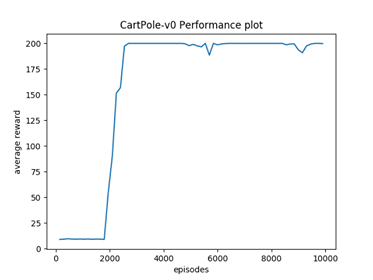
\includegraphics[scale=0.8]{Completed_Graphs/Cartpole_Single_Q.png}\\
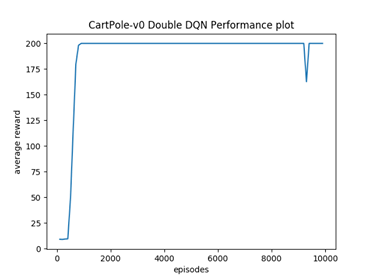
\includegraphics[scale=0.8]{Completed_Graphs/Cartpole_Double_Q.png}

Single DQN had trouble solving mountain car without significant noise in the performance graph. Double DQN had a much more stable performance with a higher end score.  This may be due to having a more stable target to train towards.
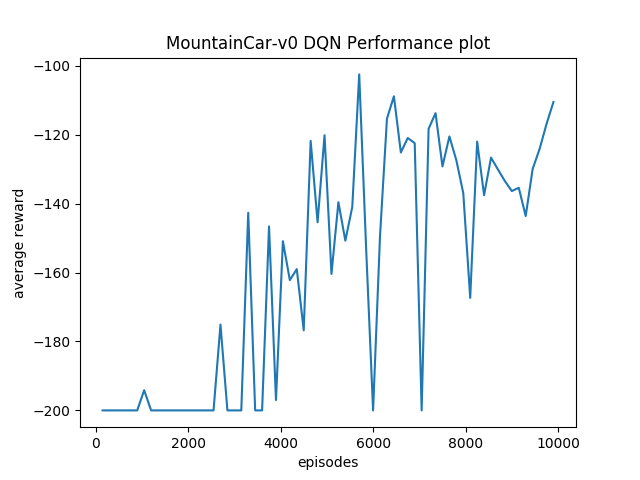
\includegraphics[scale=0.5]{Completed_Graphs/mountaincar_single_Q.png}\\
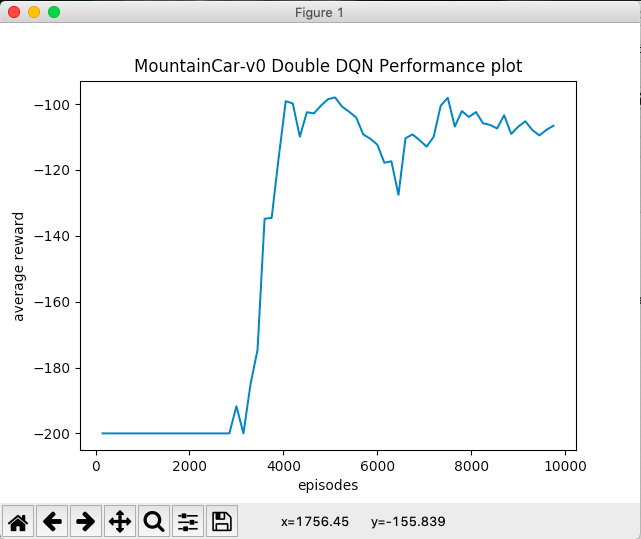
\includegraphics[scale=0.37]{Completed_Graphs/Double_DQN_performance_mountaincar.png}

The loss for Cartpole steadily increased. We hypothesize this is due to more stability, as the q-values of a cartpole state and an action given a perfect policy is not dependent on the state and action itself, but rather on the number of timesteps left until the environment returns done. For the double network, it reached perfect ignorance quickly, though unfortunately making a mistake and achieving too high loss at the end. 

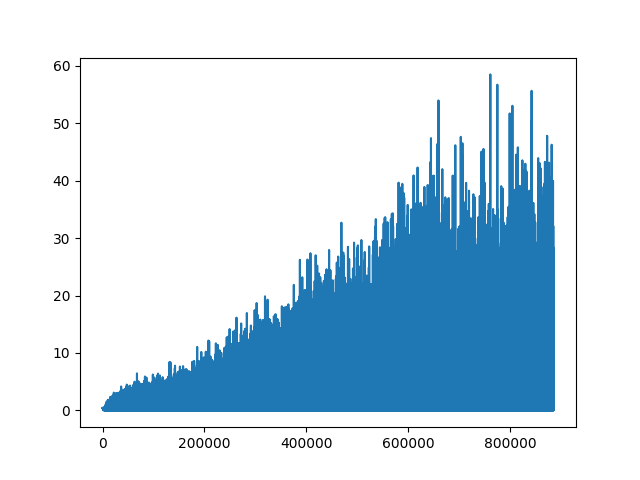
\includegraphics[scale=0.5]{Completed_Graphs/Cartpole_Single_Loss.png}\\
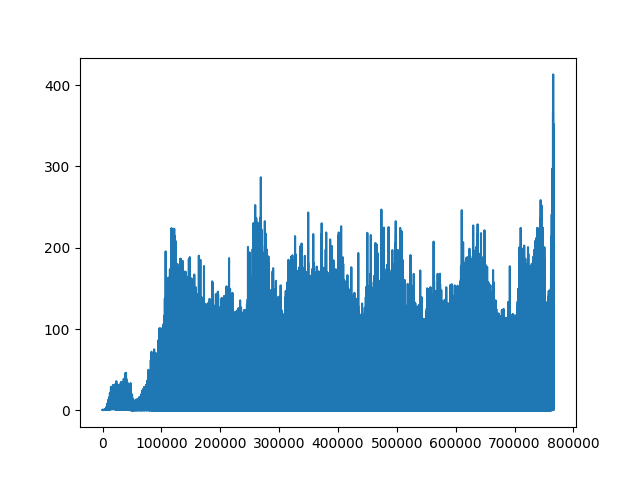
\includegraphics[scale=0.5]{Completed_Graphs/Cartpole_Double_Loss.png}\\

\section{1c and 2c}
Two step lookahead performs worse for the single DQN cartpole, with more noise in performance.This may be due to the fact that Q networks are susceptible to overestimating the value of states that are not often visited, and two step lookahead allows for taking actions that would never be taken under a greedy policy.
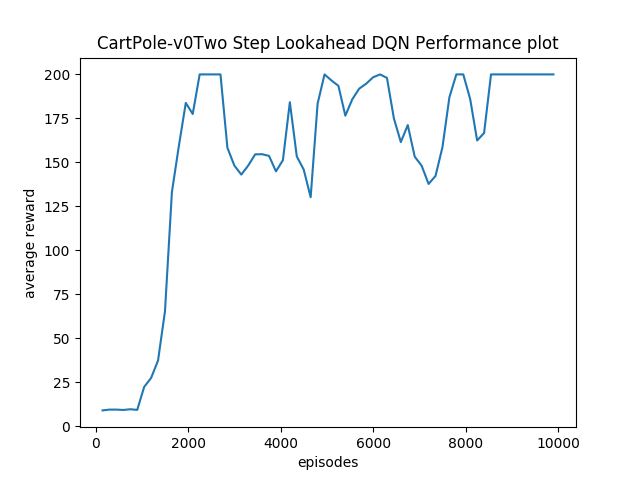
\includegraphics[scale=0.5]{Completed_Graphs/Lookahead_SingleQ.png}\\

Two step lookahead performs almost exactly as well for double DQN, due to more stable Q values\\
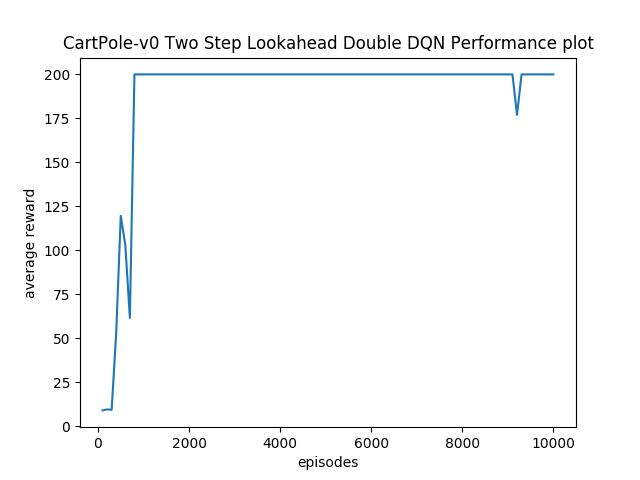
\includegraphics[scale=0.5]{Completed_Graphs/Lookahead_DoubleQ.png}\\
\section{1d and 2d}
The video-capture is in the zip, as requested.

\section{1e and 2e}
\begin{tabular}{|c|c|c|c|l}
\hline
Environment & Type & Mean & STD   \\ \hline
  CartPole & DQN  & 200  & 0   \\ \hline
  CartPole & Double DQN  & 200  & 0   \\ \hline
  Mountain Car & DQN  & -123.88  & 34.3   \\ \hline
    Mountain Car & Double DQN  & -107.35  & 8.16  \\ \hline
\end{tabular}\\

Cartpole acheived perfect performance by the end of training.  Double DQN mountain car achieved a much more consistent and higher score.  This is consistent with the general trend on the performance graphs.
\end{solution}

We recommend you to follow closely the hyperparameter setup described below.

\section*{Guidelines on references}
We recommend you to read all the papers mentioned in the references. There is a significant overlap between different papers, so in reality you should only need certain sections to implement what we ask of you. We provide pointers for relevant sections for this assignment for your convenience. \\ \\
The work in~\cite{mnih2013playing} contains the description of the experimental setup. Read paragraph~3 of section~4 for a description of the replay memory; read Algorithm~1; read  paragraphs~1 and~3 of section~4.1 for preprocessing and model architecture respectively; read section~5 for the rest of the experimental setup (e.g., reward truncation, optimization algorithm, exploration schedule, and other hyperparameters). The methods section in~\cite{mnih2015human}, may clarify a few details so it may be worth to read selectively if questions remain after reading~\cite{mnih2013playing}. \\ \\
In~\cite{van2016deep}, read "Double Q-learning"  for the definition of the double Q-learning target; read paragraph~3 of "Empirical results" for some brief comments on the experimental setup followed. \\ \\
%In~\cite{wang2015dueling}, look at equation~11 and read around three paragraphs up and down for how to set up the dueling architecture; read paragraph~2 of section~4.2 for comments on the experimental setup and model architecture. It may be worth to skim additional sections of all these papers. 

\section*{Guidelines on hyperparameters}

In this assignment you will implement improvements to the simple update Q-learning formula that make learning more stable and the trained model more performant. We briefly comment on the meaning of each hyperparameter and some reasonable values for them.
\begin{itemize}
	\item Discount factor $\gamma$: $1.$ for MountainCar, and $0.99$ for CartPole. 
	\item Learning rate $\alpha$: $0.001$ for Cartpole and $0.0001$ for Mountaincar; typically a schedule is used where learning rates get increasingly smaller. 
    \item Exploration probability $\epsilon$ in $\epsilon$-greedy: 
    While training, we suggest you start from a high epsilon value, and anneal this epsilon to a small value ($0.05$ or $0.1$) during training. 
    We have found decaying epsilon linearly from $0.5$ to $0.05$ over $100000$  iterations works well. 
    During test time, you may use a greedy policy, or an epsilon greedy policy with small epsilon ($0.05$).
    
	\item Number of training sampled interactions with the environment: 
	For MountainCar-v0, we recommend training for $3000$ to $5000$ episodes, though you should see improvements much before this. For CartPole-v0
	, you should see improvement around $2000$ episodes. However, for the plots, report the training curve for $10000$ episodes.
	
	Look at the average reward achieved in the last few episodes  to test if performance has plateaued; it is usually a 
    good idea to consider reducing the learning rate or the exploration 
	probability if performance plateaus.
 	
 	\item Replay buffer size: $50000$; 
	this hyperparameter is used only for experience replay. It determines how many of the last transitions experienced you will keep in the replay buffer before you start rewriting this experience with more recent transitions.
	
	\item Batch size:  32;  typically, rather doing the update as in (2), we use a small batch of sampled experiences from the replay buffer; this provides better hardware utilization.
\end{itemize}

In addition to the hyperparameters you also have the choice of which
optimizer and which loss function to use. We recommend you use Adam as
the optimizer. It will automatically adjust the learning rate based on
the statistics of the gradients its observing. Think of it like a
fancier SGD with momentum. Both Tensorflow and Keras provide versions
of Adam.

For the loss function, you can use Mean Squared Error. 

The implementations of the methods in this homework have multiple
hyperparameters.  These hyperparameters (and others) are part of the
experimental setup described in~\cite{mnih2013playing, mnih2015human}.
For the most part, we strongly suggest you to follow the experimental
setup described in each of the papers.  \cite{mnih2013playing,
  mnih2015human} was published first; your choice of hyperparameters
and the experimental setup should follow closely their setup.
%\cite{van2016deep, wang2015dueling} follow for the most part the setup
%of \cite{mnih2013playing, mnih2015human}.  
We recommend you to read
all these papers.  We have given pointers for the most relevant portions for
you to read in a previous section.

\section*{Guidelines on implementation}

This homework requires a significant implementation effort. It is hard to read through the papers once and know immediately what you will need to be implement. We suggest you to think about the different components (e.g., replay buffer, Tensorflow or Keras model definition, model updater, model runner,
exploration schedule, learning rate schedule, ...) that you will need to implement for each of the different methods that we ask you about, and then read through the papers having these components in mind. By this we mean that you should try to divide and implement small components with well-defined functionalities rather than try to implement everything at once. Much of the code and experimental setup is shared between the different methods so identifying well-defined reusable components will 
save you trouble. We provide some code templates that you can use if you wish. Contrary to the previous assignment, abiding to the function signatures defined in these templates is not mandatory you can write your code from scratch if you wish. 

Please note, that while this assignment has a lot of pieces to implement, most of the algorithms you will use in your project will be using the same pieces. Feel free to reuse any code you write for your
homeworks in your class projects.


This is a challenging assignment. 
\textbf{Please start early!}

\nocite{*}
\bibliographystyle{plain}
\bibliography{deeprlhw2}

\end{document}

